\documentclass[journal]{vgtc}                % final (journal style)
%\documentclass[review,journal]{vgtc}         % review (journal style)
%\documentclass[widereview]{vgtc}             % wide-spaced review
%\documentclass[preprint,journal]{vgtc}       % preprint (journal style)

%% Uncomment one of the lines above depending on where your paper is
%% in the conference process. ``review'' and ``widereview'' are for review
%% submission, ``preprint'' is for pre-publication, and the final version
%% doesn't use a specific qualifier.

%% These few lines make a distinction between latex and pdflatex calls and they
%% bring in essential packages for graphics and font handling.
%% Note that due to the \DeclareGraphicsExtensions{} call it is no longer necessary
%% to provide the the path and extension of a graphics file:
%% 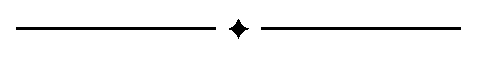
\includegraphics{diamondrule} is completely sufficient.
%%
\ifpdf%                                % if we use pdflatex
  \pdfoutput=1\relax                   % create PDFs from pdfLaTeX
  \pdfcompresslevel=9                  % PDF Compression
  \pdfoptionpdfminorversion=7          % create PDF 1.7
  \ExecuteOptions{pdftex}
  \usepackage{graphicx}                % allow us to embed graphics files
  \DeclareGraphicsExtensions{.pdf,.png,.jpg,.jpeg} % for pdflatex we expect .pdf, .png, or .jpg files
\else%                                 % else we use pure latex
  \ExecuteOptions{dvips}
  \usepackage{graphicx}                % allow us to embed graphics files
  \DeclareGraphicsExtensions{.eps}     % for pure latex we expect eps files
\fi%

%% it is recomended to use ``\autoref{sec:bla}'' instead of ``Fig.~\ref{sec:bla}''
\graphicspath{{figures/}{pictures/}{images/}{./}} % where to search for the images

\usepackage{microtype}                 % use micro-typography (slightly more compact, better to read)
\PassOptionsToPackage{warn}{textcomp}  % to address font issues with \textrightarrow
\usepackage{textcomp}                  % use better special symbols
\usepackage{mathptmx}                  % use matching math font
\usepackage{times}                     % we use Times as the main font
\renewcommand*\ttdefault{txtt}         % a nicer typewriter font
\usepackage{cite}

%% If you are submitting a paper to a conference for review with a double
%% blind reviewing process, please replace the value ``0'' below with your
%% OnlineID. Otherwise, you may safely leave it at ``0''.
\onlineid{0}

%% declare the category of your paper, only shown in review mode
\vgtccategory{Research}

%% Paper title - 1 pt for descriptive title
\title{Title}

%% This is how authors are specified in the journal style

%% indicate IEEE Member or Student Member in form indicated below
%% 1 pt for name
\author{Author}
\authorfooter{
%% insert punctuation at end of each item
\item
 Author is a student at the University of Arizona. E-mail: email8@email.arizona.edu.
}

%other entries to be set up for journal
%\shortauthortitle{Firstauthor \MakeLowercase{\textit{et al.}}: Paper Title}

%% Abstract section - 5 pts
\abstract{
The goal of this project is to...

} % end of abstract

%% Keywords that describe your work. Will show as 'Index Terms' in journal
%% please capitalize first letter and insert punctuation after last keyword
%\keywords{Radiosity, global illumination, constant time}

%% ACM Computing Classification System (CCS).
%% See <http://www.acm.org/class/1998/> for details.
%% The ``\CCScat'' command takes four arguments.

%\CCScatlist{ % not used in journal version
% \CCScat{K.6.1}{Management of Computing and Information Systems}%
%{Project and People Management}{Life Cycle};
% \CCScat{K.7.m}{The Computing Profession}{Miscellaneous}{Ethics}
%}

%% Uncomment below to include a teaser figure.
%   \teaser{
%   \centering
%   \includegraphics[width=16cm]{CypressView}
%   \caption{In the Clouds: Vancouver from Cypress Mountain.}
%  }

%% Uncomment below to disable the manuscript note
%\renewcommand{\manuscriptnotetxt}{}

%% Copyright space is enabled by default as required by guidelines.
%% It is disabled by the 'review' option or via the following command:
% \nocopyrightspace

\vgtcinsertpkg

%%%%%%%%%%%%%%%%%%%%%%%%%%%%%%%%%%%%%%%%%%%%%%%%%%%%%%%%%%%%%%%%
%%%%%%%%%%%%%%%%%%%%%% START OF THE PAPER %%%%%%%%%%%%%%%%%%%%%%
%%%%%%%%%%%%%%%%%%%%%%%%%%%%%%%%%%%%%%%%%%%%%%%%%%%%%%%%%%%%%%%%%

\begin{document}

%% The ``\maketitle'' command must be the first command after the
%% ``\begin{document}'' command. It prepares and prints the title block.

%% the only exception to this rule is the \firstsection command
\firstsection{Introduction} % or "Motivation"

\maketitle

% Introduction and/or Motivation - 20%

We demonstrate...

This problem is important because...

To solve this problem, we...

% You may want to end this section by summarizing it again as a list, for example:
% The aims of this research are:
% \begin{itemize}
%   \item categorize different types of visual embellishments
%   \item analyze and redefine the term "chartjunk"
%   \item determine which visual embellishments are more effective for the memorability and comprehensibility of charts
% \end{itemize}


%Background and Related Work: 20%

\section{Background}
\label{sec:background}

This work is relevant to any domain...
~\cite{Bateman:2015:Junk}

\subsection{Related Work}
\label{sec:related}

There is a lot of preexisting work surrounding...

% \begin{figure}[h]
%  \centering % avoid the use of \begin{center}...\end{center} and use \centering instead (more compact)
%  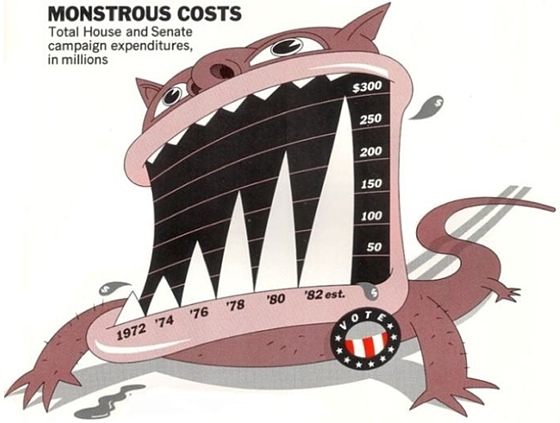
\includegraphics[width=2in]{figs/holmes}
%  \caption{An example of chartjunk with Holmes' visually embellished charts.}
%  \label{fig:holmes}
% \end{figure}


%Research Plan - 20%
\section{Research Plan}
\label{sec:research}

We are solving the problem surrounding...

\subsection{Data}
\label{sec:data}

The data...

\subsection{Evaluation}
\label{sec:eval}

To evaluate our work...

\subsection{Technology}
\label{sec:tech}

We used...


% Impact - 20%
\section{Impacts}
\label{sec:impact}

This project provides more information regarding...


%\bibliographystyle{abbrv}
\bibliographystyle{abbrv-doi-hyperref}
%%use following if all content of bibtex file should be shown
%\nocite{*}
\bibliography{update}
\end{document}
